\documentclass{article}
\usepackage[utf8]{inputenc}

\title{\Huge\textbf{Formal Modeling of ShopAdvizor in VDM++}\linebreak\linebreak\linebreak
\Large\textbf{Report}\linebreak
\linebreak\linebreak

\includegraphics[scale=0.1]{feup.png}\linebreak\linebreak
\linebreak\linebreak
\Large{Métodos Formais em Engenharia de Software}
\linebreak\linebreak
}

\author{\textbf{Class 3 Group 3}\\
Daniel Filipe Santos Marques - up201503822@fe.up.pt \\ Maria Eduarda Santos Cunha - up201506524@fe.up.pt
\\\linebreak\linebreak
\vspace{1cm}}

\usepackage{natbib}
\usepackage{graphicx}

\begin{document}

\maketitle

\newpage
\tableofcontents
\newpage

\section{Informal System Description and List of Requirements}
\subsection{Informal System Description}
aaaaa
\subsection{List of Requirements}
\begin{table}[h]
\begin{tabular}{|p{1cm}|p{2cm}|p{8cm}|}
\hline
\textbf{Id} & \textbf{Priority} & \textbf{Description} \\
\hline
R1          & Mandatory          & A user may view products' information provided by other users, which includes reviews, ratings and composition \\
\hline
R2          & Mandatory          & A user may add a review and rating to an existing product\\
\hline
R3          & Mandatory          & A user may add new products to be reviewed \\
\hline
R4          & Mandatory          & A user may add ingredients and their quantities to a product
\\
\hline
R5          & Mandatory          & A user may search for products by name, brand or retailer \\
\hline
R6          & Optional          & A user may delete a review \\
\hline
\end{tabular}
\end{table}
These requirements were directly translated onto use cases shown in the section Visual UML Model, Use Case Model.

\section{Visual UML Model}

\subsection{Use Case Model}
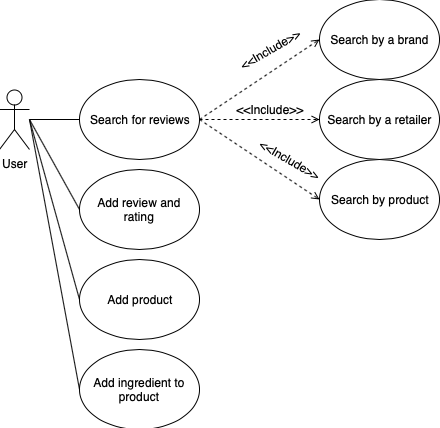
\includegraphics[scale=0.8]{usecasemodel.png}\linebreak\linebreak

The major use case scenarios which will be used later as test scenarios are described next.

\begin{table}[!h]
\begin{tabular}{|p{3cm}|p{8cm}|}
\hline
\textbf{Scenario} & \textbf{AAAA} \\
\hline
\textbf{Description}          & aaaa \\
\hline
\textbf{Pre-conditions}       & aaaa \\
\hline
\textbf{Post-conditions}      & aaaa \\
\hline
\textbf{Steps}                & aaaa \\
\hline
\textbf{Exceptions}           & aaaa \\
\hline
\end{tabular}
\end{table}

\subsection{Class Model}
\begin{table}[h]
\begin{tabular}{|p{3cm}|p{8cm}|}
\hline
\textbf{Class} & \textbf{Description} \\
\hline
Activity           & aaa \\
\hline
Brand              & Defines a brand which is attributed to a product. \\
\hline
Competition        & aaa \\
\hline
Product            & Defines a product in the system to be reviewed. \\
\hline
Retailer           & Defines a retailer responsible for the sale of a product. \\
\hline
ShopAdvizor        & Core model; Defines the main system where all elements are initialized or added. \\
\hline
ShopAdvizorTest    & Class where tests are implemented. \\
\hline
User               & Defines a user who may view products' reviews, add their own reviews and partake on missions. \\
\hline
\end{tabular}
\end{table}

\section{Formal VDM++ Model}
\subsection{Class Activity}
aaaaa
\subsection{Class Brand}
aaaaa
\subsection{Class Competition}
aaaaa
\subsection{Class Product}
aaaaa
\subsection{Class Retailer}
aaaaa
\subsection{Class ShopAdvizor}
aaaaa
\subsection{Class User}
aaaaa

\section{Model Validation}
\subsection{Class ShopAdvizorTest}
aaaaa

\section{Model Verification}
\subsection{Example of Domain Verification}
aaaaa
\subsection{Example of Invariant Verification}
aaaaa

\section{Code Generation}
aaaaa

\section{Conclusions}
The model we developed not only covers all the requirements set in the provided guidelines but also accommodates additional features we created with the purpose of adding complexity to the project and allowing us to explore VDM++ in more depth.
Although we are pleased with the end result, in the future we believe we could add even more features as to make use of 
This project took approximately x hours to develop, all operations and tests included.

\section{References}
\begin{enumerate}  
\item Overture tool web site, http://overturetool.org
\item VDM-10 Language Manual, Peter Gorm Larsen et al, Overture Technical Report Series No. TR-001, March 2014
\item Class slides on VDM++ 
\end{enumerate}

\end{document}